%Tablas hechas con la herramienta http://www.tablesgenerator.com/# cambiando l para p{8cm} para hacer el salto de linea
\documentclass{article}

\usepackage{titlesec}
\usepackage[utf8]{inputenc}
\usepackage{graphicx}
\usepackage{ amssymb }
%\usepackage{subfig}
\usepackage{subcaption}
%\usepackage{breqn}
\usepackage{mathtools,bm}
\usepackage{eurosym}
\usepackage{amstext} % for \text
\DeclareRobustCommand{\officialeuro}{%
  \ifmmode\expandafter\text\fi
  {\fontencoding{U}\fontfamily{eurosym}\selectfont e}}
\usepackage[spanish]{babel} %changes the LaTex default labels to spanish
\usepackage{float} %enables the anchorage of the figures and tables within the text, with [H]
\usepackage{longtable}

\usepackage[a4paper,bindingoffset=0.2in,%
            left=1in,right=1in,top=1in,bottom=1in,%
            footskip=.25in]{geometry}
% \graphicspath{ {images/}, {images2/} }
\usepackage{amsmath}
\usepackage[hyphens]{url}
\usepackage{hyperref}
\usepackage{multirow}


%\setcounter{secnumdepth}{4}

\titleformat{\paragraph}
{\normalfont\normalsize\bfseries}{\theparagraph}{1em}{}
\titlespacing*{\paragraph}
{0pt}{3.25ex plus 1ex minus .2ex}{1.5ex plus .2ex}

\newcommand*{\frontPageEC}[2]{
    \begingroup % Create the command for including the title page in the document
        \centering % Center all text
        \vspace*{\baselineskip} % White space at the top of the page
        {\begin{flushright} \LARGE #1  \end{flushright}}
        \vspace*{\baselineskip}
        \rule{\textwidth}{1.6pt}\vspace*{-\baselineskip}\vspace*{2pt} % Thick horizontal line
        \rule{\textwidth}{0.4pt}\\[\baselineskip] % Thin horizontal line
        {\LARGE #2  \\[0.8\baselineskip] \large{Robótica y Percepción Computacional}}\\[0.2\baselineskip] % Title
        \rule{\textwidth}{0.4pt}\vspace*{-\baselineskip}\vspace{3.2pt} % Thin horizontal line
        \rule{\textwidth}{1.6pt}\\[\baselineskip] % Thick horizontal line
        \vspace*{2\baselineskip} % Whitespace between location/year and editors
        Alumnos: \\[\baselineskip]
        {\Large Luciano García Giordano (150245)} \\
        {\Large Gonzalo Flórez Arias (150048)} \\
        {\Large Salvador González Gerpe (150044)} \\
        
        \vfill
        %\includegraphics[scale=0.4]{UPM.png}
        
        {\itshape Universidad Politécnica de Madrid \\ ETSI Informáticos\par} % Editor affiliation
    \endgroup}

\title{Control entrega}
\author{Luciano García Giordano, Gonzalo Flórez Arias, Salvador González Gerpe}
\date{01/03/2019}
\date{Universidad Politécnica de Madrid}
\begin{document}

\frontPageEC{01 de marzo de 2019}{Entrega 01: Control}
\thispagestyle{empty}

\newpage
\tableofcontents
\setcounter{page}{1}

\clearpage
\newpage



\section{Descripción del programa}
Partiendo del programa Brain base del robot proporcionado por el profesorado de la asignatura, se han implementado una serie de cambios y mejoras, teniendo en mente 3 objetivos principales: lograr que el robot encuentre inicialmente la línea y sea capaz de recuperarla en caso de perderla; asegurar que el recorrido y velocidad del robot sobre la línea sean máximos; permitir que el robot esquive obstáculos mediante el uso de sus sónares (asegurando que deje y retome la línea correctamente al encontrarse con un obstáculo).

Por un lado, se planteó la necesidad de procurar que el robot encuentre la línea inicialmente. En este sentido, aunque es probable que se puedan encontrar soluciones mejores, nuestro código se limita a avanzar hacia adelante hasta que encuentre la línea, tras lo cual comienza el acercamiento progresivo (explicado en detalle en el siguiente apartado. Por otro lado, una vez que el robot pierda la línea, irá hacia atrás. En este sentido, nos dimos cuenta inicialmente de que a veces al volver atrás estaba girando demasiado, y le costaba volver a la línea de la que se escapó. Por tanto, está implementada una marcha atrás similar al aparcar en paralelo con un coche: si se ha salido hacia la izquierda de la línea, comienza dando marcha atrás hacia la derecha, para posteriormente dar marcha atrás a la izquierda y así reorientarse para estar lo más cerca posible de estar posicionado sobre la línea, con lo que pueda reanudar su marcha sin inconvenientes. De esa manera, volvemos recorriendo aquello que se asemejaría a una ''S'', de forma que el robot siempre encuentra la línea tras perderla. En curvas muy cerradas, eso es especialmente útil, aunque puede causar que el robot cambie el sentido de la marcha tras ''encontrar la línea'' por la que venía.

Respecto al propio código que afecta al acercamiento a la línea y su recorrido sobre ella, inicialmente se trató de implementar los distintos Kp, Kd y Ki vistos en clase, para luego entender qué valores para los mismos serían los idóneos para lograr que el recorrido sea óptimo. A este respecto, consideramos óptimo que cuanto más lejos esté de a línea, más rápida y pronunciadamente se acerque. Cuanto más se acerca, su velocidad y giro debe ir reduciéndose, ya que no es ideal que sobrepase la línea demasiado, pues acabaría haciendo simplemente zigzags en vez de ir lo más recto posible por la línea. Tras ir probando distintas opciones, pensamos que podríamos realizar un modelo cuadrático en Kd, pues parece tener sentido generar, a partir de un par de parámetros, una parábola que modelice bien la velocidad de movimiento según la distancia a la línea. Kp se queda haciendo referencia al ángulo de giro. Para poder encontrar los parámetros, se usó el software Geogebra, en el cuál generamos una parábola y mediante los parámetros ''a'' y ''b'' (luego introducidos en el código), fuimos probando hasta encontrar una curva que nos satisficiese. Hemos probado también el uso de Ki, pero dado que no tenemos un sistema en que la aceleración tiene demasiada importancia pierde el sentido su uso. De esa manera, preferimos no usarlo, ya que sería una complejidad añadida sobre un robot que recorre bien la línea sin necesitar ese parámetro.

% [Aquí meter foto del modelo cuadrático]

\begin{figure}[H]
    \centering
    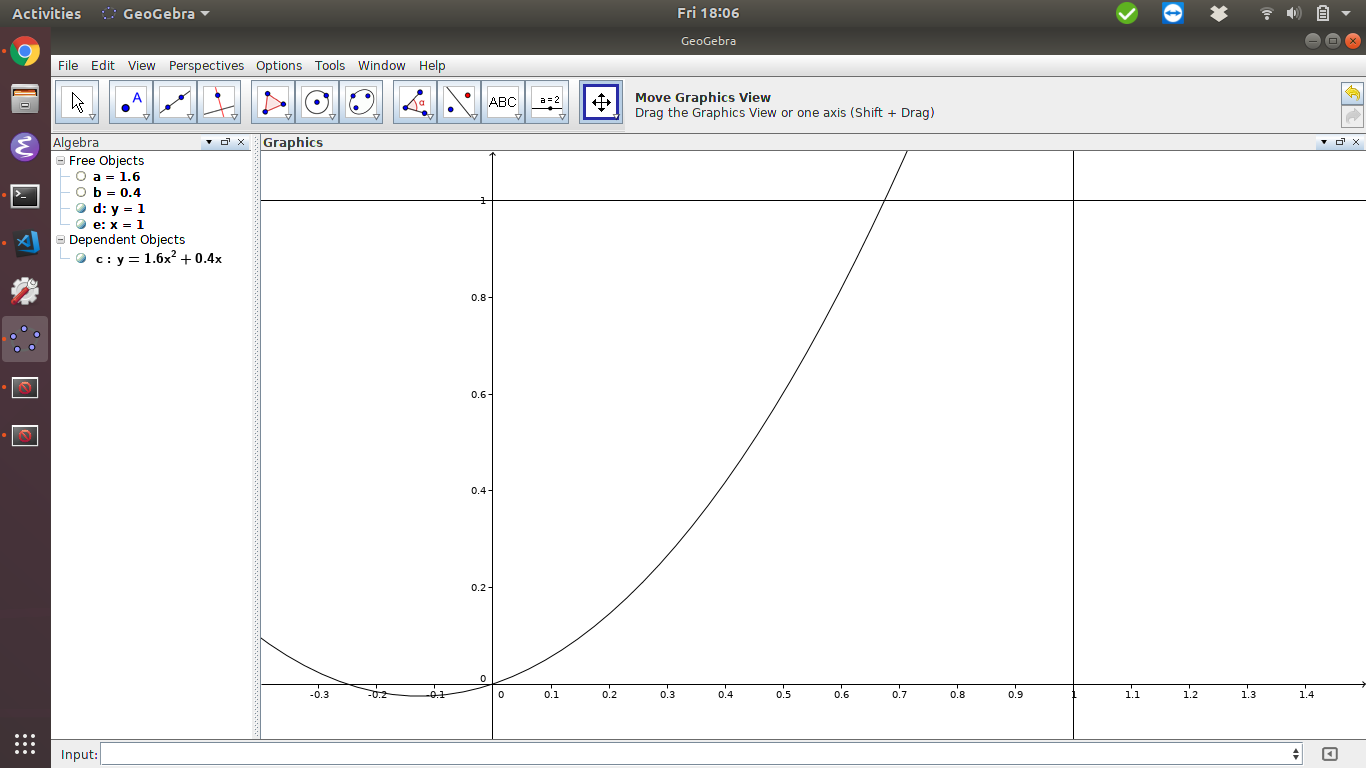
\includegraphics[width=12cm]{modeloCuadratico.png}
    \caption{Observamos el modelo cuadrático en el software GeoGebra para determinar los parámetros iniciales para nuestra exploración. Con el simulador, los hemos cambiado según nuestras observaciones para que fuera más adecuado al funcionamiento del robot.}
    \label{fig:modeloCuadratico}
\end{figure}

Basándonos tanto en el sistema de seguir paredes que ya desarrollamos para la primera tarea de la asignatura como en el estado de seguir líneas de esta entrega, implementamos la capacidad del robot de emplear sus sónares para encontrar y esquivar obstáculos que se interpongan en su camino. En este caso, calculamos la distancia respecto al objeto de tal manera que es positiva si está más lejos de cierta distancia $d$ del objeto, y negativa si está más cerca de lo deseado. De esa manera, tenemos una trayectoria virtual, que podemos recorrer como si fuera una línea, alrededor del objeto. Para poder intentar desviar mejor los obstáculos, implementamos nuestra solución en dos casos posibles: que el obstáculo esté más cerca del lado izquierdo del robot, o del lado derecho. Si se da el primer caso, el robot tratará de virar hacia la derecha, siguiendo a su izquierda el obstáculo cual pared a recorrer, y bordeándola hasta que encuentre de nuevo la línea. Entonces, el robot olvidará su tarea de seguir el obstáculo, y retomará la línea. Si se da el segundo caso comentado el resultado es análogo. Se añadió además un limitador de la velocidad máxima mientras sigue la línea según la distancia de cualquier objeto para asegurar que el robot no avance demasiado antes de decidir que está en ruta de colisión con un objeto. Nuestro objetivo con eso era evitar choques con los obstáculos al virar cuando intenta rodearlo.

\subsection{Modelo utilizado}

En resúmen, hemos implementado un robot que tiene una serie de estados y transiciones entre estados, organizados de la siguiente manera:

\begin{itemize}
    \item \textbf{initialSearchLine}: avanza hacia delante buscando una línea. Transita a followLine cuando la encuentra. Transita a circleObjectOnRight o a circleObjectOnLeft si encuentra un objeto por delante.
    \item \textbf{searchLine}: intenta encontrar la línea yendo hacia atrás en forma de ''S''. Transita a followLine cuando la encuentra.
    \item \textbf{approachLine}: sirve para aproximarse a una línea sin que otras variables le afecten. Transita a followLine cuando está cerca de la línea.
    \item \textbf{followLine}: sigue la línea implementando la consigna que lleva $K_d$ y $K_p$ en consideración. Transita a circleObjectOnLeft o a circleObjectOnRight cuando encuentra un obstáculo (dependiendo de por qué lado le encuentra).
    \item \textbf{circleObjectOnRight y circleObjectOnLeft}: circulan el objeto utilizando la consigna descrita anteriormente. Básicamente sique una línea virtual calculada a partir de la distancia al objeto. Transita a leaveObjectOnRight o a leaveObjectOnLeft (respectivamente) cuando encuentra una línea más cerca de 0.3 unidades.
    \item \textbf{leaveObjectOnRight y leaveObjectOnLeft}: dejan de seguir el objeto y hacen una curva en la dirección adecuada para seguir la línea anteriormente encontrada. Transita a approachLine cuando encuentra una línea a menos de 0.95 unidades.
\end{itemize}

\section{Ejemplos ejecutados}
Se muestran a continuación los tests con los que se ha probado el robot, incluyendo la traza en rojo del recorrido del mismo sobre el mapa.

% [Incluir los mapas]
Con el background 1 desarrollamos todo el modelo de funcionamiento. Llegamos a una solución para nosotros aceptable, que se muestra en la figura \ref{fig:mapa1}. La optimización de los parámetros también se decidieron en su mayoría en este mapa.

\begin{figure}[H]
    \centering
    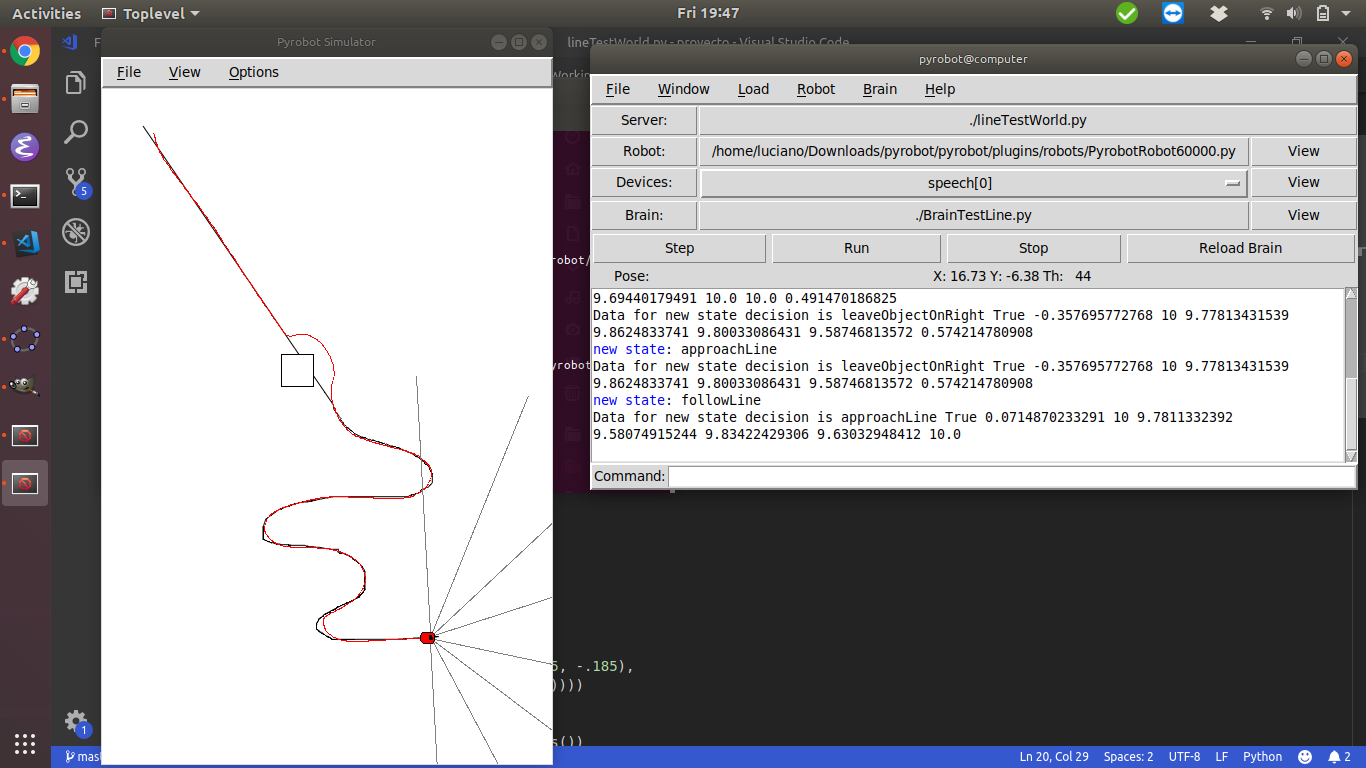
\includegraphics[width=12cm]{mapa1.png}
    \caption{Uno de los resultados con el background 1.}
    \label{fig:mapa1}
\end{figure}

Ya en el background 2, hicimos tanto cambios en los parámetros como desafíos más complejos con los objetos. Pudimos observar que faltaban estados para las salidas de los objetos, y los añadimos y probamos en este y en el anterior backgrounds.

\begin{figure}[H]
    \centering
    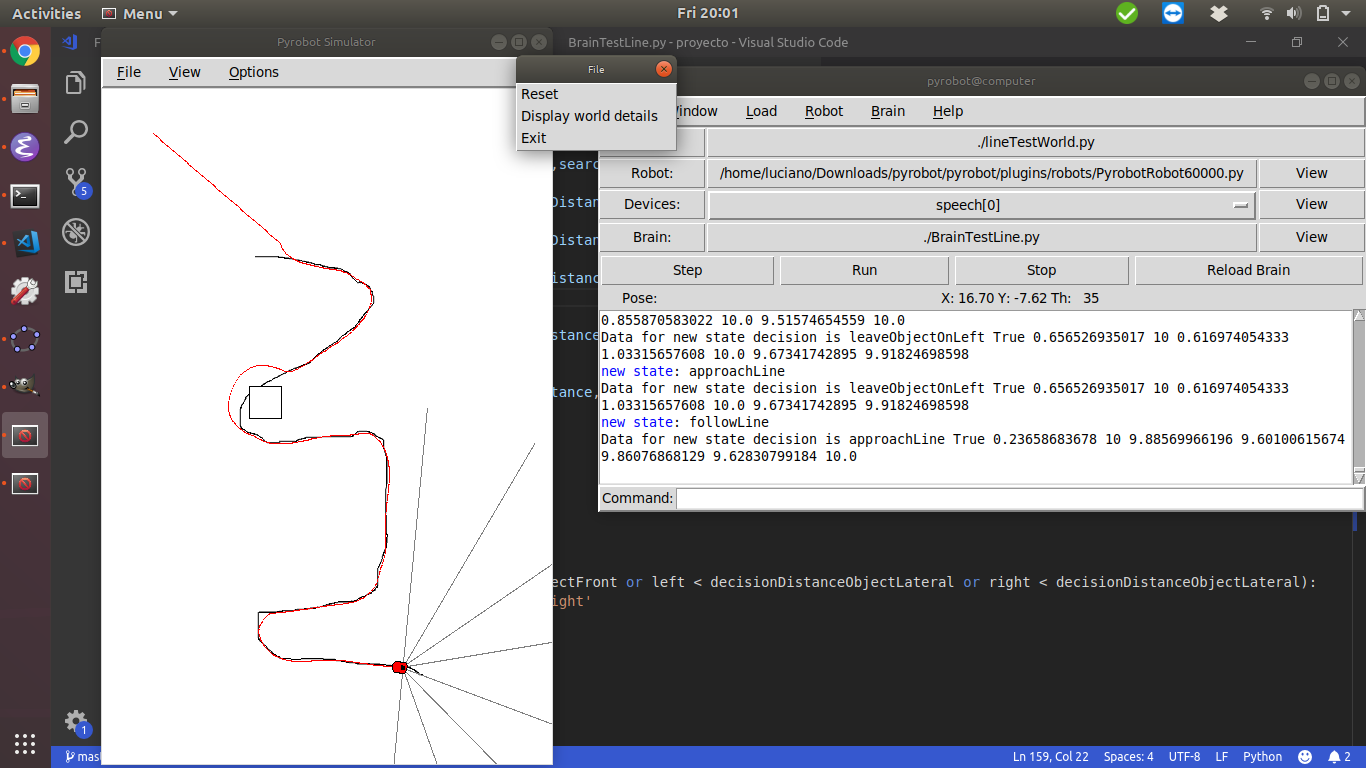
\includegraphics[width=12cm]{mapa2_1.png}
    \caption{Con el background 2 probamos soluciones más complejas, y con más objetos.}
    \label{fig:mapa2}
\end{figure}

\begin{figure}[H]
    \centering
    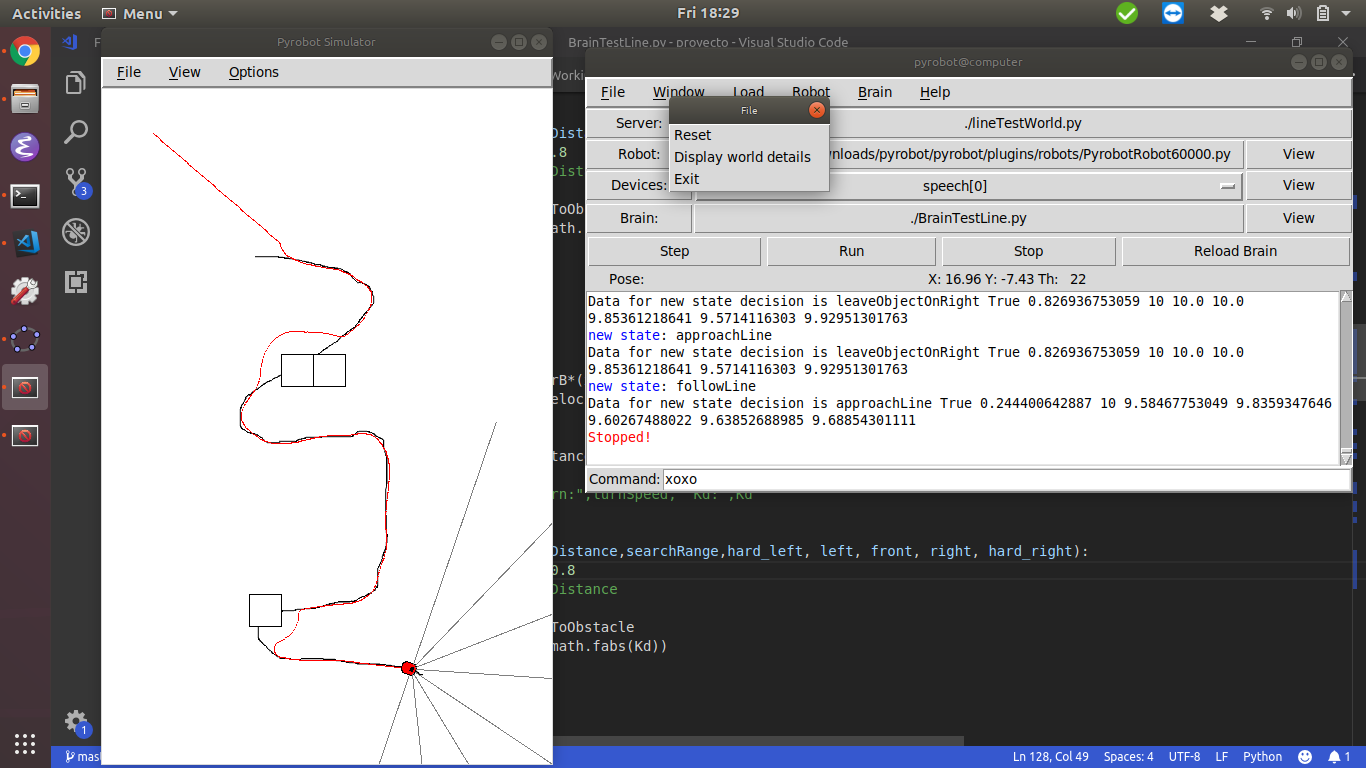
\includegraphics[width=12cm]{mapa2.png}
    \caption{Otro resultado con el background 2.}
    \label{fig:mapa2_1}
\end{figure}

En el background 3, de invención nuestra, hicimos un circuito cerrado. En diversas ocasiones, conseguimos hacer que el robot hiciera la vuelta entera (incluyendo las cerradas curvas de la derecha). Sin embargo, por un problema conocido del simulador, en muchos casos se queda atascado en un objeto porque el simulador no detecta la línea. En la salida por texto del programa en la figura \ref{fig:mapa3}, podemos observar varios ''False'', que corresponden justamente a no detectar la línea (variable hasLine).

% [Mapa del error línea perpendicular]
\begin{figure}[H]
    \centering
    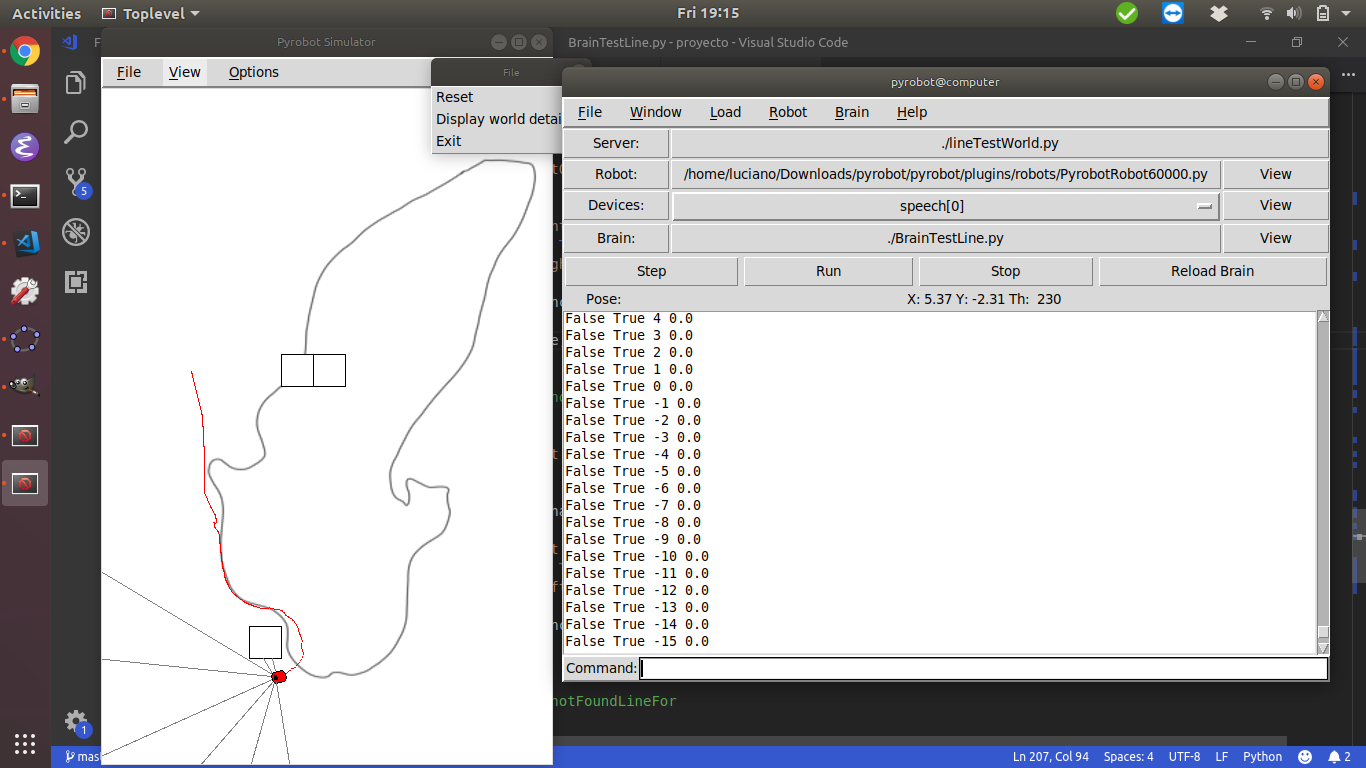
\includegraphics[width=12cm]{mapa3.png}
    \caption{El simulador no detecta bien las líneas cuando están en perpendicular.}
    \label{fig:mapa3}
\end{figure}

Como se puede observar, en algunos casos no se logra retomar la línea tras rodear un obstáculo debido al simulador, por el tema de que al encontrarse una línea perpendicular delante  no encuentra correctamente la distancia del centro, y por lo tanto no avisa al robot de que deje de seguir el obstáculo y vuelva a reencontrarse con la línea.


Ya en el background 4, quisimos comprobar la capacidad del robot de completar un circuito cerrado. Elegimos para ello el conocido circuito de Hockenheim, llamado Hockenheimring \cite{hockenheimring}. Pusimos un objeto en la curva más cerrada dado que era demasiado cerrada.

\begin{figure}[H]
    \centering
    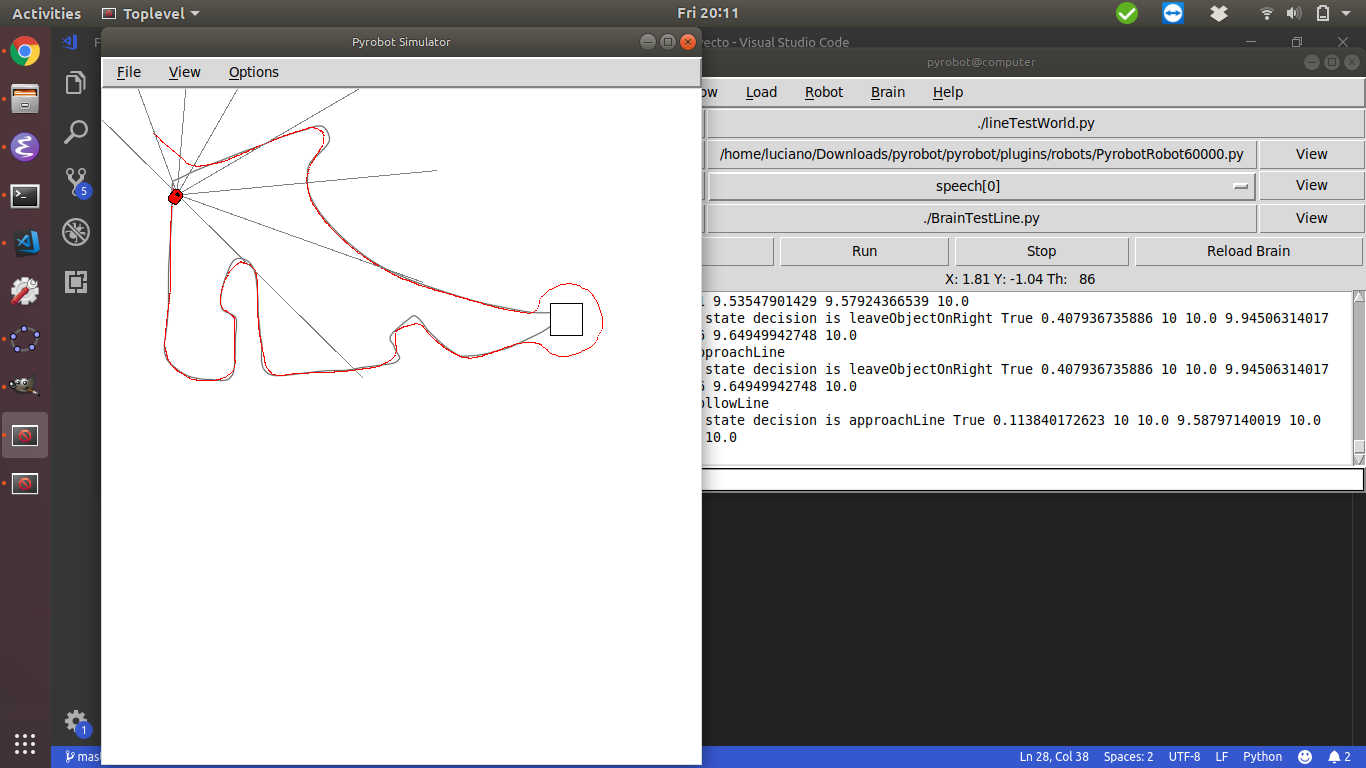
\includegraphics[width=12cm]{mapa4.png}
    \caption{Hockenheimring. El robot es capaz de dar una vuelta completa en el circuito.}
    \label{fig:mapa4}
\end{figure}

Como podemos observar, el robot entra en el circuito, lo recurre entero, da la vuelta alrededor del objeto y lo completa. En la ejecución mostrada en la figura \ref{fig:mapa4}, más adelante el robot finalizó la vuelta. Y no solo finalizó la vuelta como fue capaz de hacer una más antes que paráramos la simulación. De la manera que estaba funcionando, es muy probable que si hubiéramos dejado el simulador funcionando conseguiríamos más vueltas. 


\begin{thebibliography}{1}

    \bibitem{hockenheimring} Hockenheimring Official Website. (n.d.). Retrieved March 1, 2019, from https://www.hockenheimring.de/en

\end{thebibliography}












% \section{Introducción}
%     Esta práctica se centra en la implementación y análisis de dos sencillos algoritmos de clustering, uno de ellos quizás menos explorado por su ineficiencia computacional, el algoritmo de clustering secuencial, y el otro ampliamente utilizado, el algoritmo de las k-medias.

%     El objetivo es implementar y comparar los algoritmos propuestos para los datasets Iris, Wine, Cancer, Isolet y MNIST, disponibles en el aula virtual de la asignatura. La finalidad es que se puedan comparar la forma con que son capaces de hacer la separación de los datos en diferentes agrupaciones, también llamadas \textit{clusters}. Para ello, implementaré los dos algoritmos y utilizaré también de implementaciones disponibles en bibliotecas como scikit-learn. Además, se analizará la capacidad de indicación de sugerencia de número de clusters mediante el uso de la técnica chainmap.

% \section{Algoritmo de las k-medias}
%     El algoritmo de las k-medias se basa en la distancia entre cada instancia y un representante de grupo para separar las instancias disponibles en un número predefinido (k) de grupos. Inicialmente, el algoritmo asigna a $k$ instancias aleatorias para que sean centroides de cada uno de esos $k$, clusters. A partir de ese momento, ejecuta hasta la estabilidad de los clusters (o hasta que pase cierto número de iteraciones) la siguiente secuencia:

%     En el paso 1, para cada $x_{i}$, se asigna el cluster $j$ cuyo centroide es $c_{j}$:

%     $$\alpha_{i}=\arg\min_{j}\left\{ d_{E} \left( x_{i}, c_{j} \right) \right\}$$

%     Tras asignar todos los clusters, en el paso 2 se actualizan los centroides según la siguiente ecuación:

%     $$C_{j} = \left\{ x_{i}\vline \alpha _{i}=j\right\}$$

%     $$c_{j}=\dfrac {\sum _{X\in Cj}X}{N\left( C_{j}\right) }$$

%     Cuando el algoritmo llega a la estabilidad o es terminado por exceder el número de iteraciones máximo, llegamos idealmente a una separación en $k$ clusters.

%     Sin embargo, dicha separación no siempre es perfecta según lo que esperamos inicialmente. Y hay muchas razones para ello, algunas listadas:
%     \begin{itemize}
%         \item El número $k$ de clusters puede no corresponder con el número de ''clases'' (o el número de categorías de cosas.
%         \item El algoritmo puede no conseguir modelar bien las relaciones entre las variables que definen la categoría de cada objeto. Por ejemplo, el k-medias, basado en la distancia euclidea, no es capaz de hacer cluster sobre objetos en que las relaciones cuadráticas entre ciertas variables son muy importantes.
%         \item Podemos tener un dataset en que lo que definimos como instancias de diferentes categorías se representan en las variables con medidas no tan diferentes o con relaciones difusas. En este caso, decimos que hay solape entre clases. Son necesarias nuevas, diferentes o más bien medidas variables para que los clusters sean más bien separables.
%     \end{itemize}

%     \subsection{Chainmap}
%         Para definir un número previo de clusters en los que intentar separar los datos de cada dataset, evaluamos con el procedimiento llamado Chainmap cada uno de los datasets, esperando a través de ello poder decir aproximadamente cuántos clusters tenemos disponibles en el dataset.

%         Dicho algoritmo elige una instancia del dataset aleatoriamente. Y a partir de esa instancia, hasta que no queden más, elige aquella cuya distancia a partir de la anterior es mínima. Elimina dicha instancia y registra la distancia medida. Vuelve al segundo paso, buscando por el siguiente punto que minimice la distancia.

%         El resultado es un algoritmo que genera una gráfica que idealmente mostraría, a través de picos de distancia, los diferentes clusters presentes. Sin embargo, varias son las razones que pueden causar que dicha gráfica no demuestre el número adecuado de picos. Se listan algunas de las razones a seguir:
%         \begin{itemize}
%             \item Hay datasets en los que la distancia euclídea no tiene sentido. Por ejemplo, cuando las relaciones entre las variables son de naturaleza cuadrática o exponencial. En este caso, puede parecer más cerca una instancia que en realidad pertenece a otro grupo porque la distancia es lineal, que otra instancia más similar pero que se sitúa en una distancia euclídea inferior.
%             \item Para ciertos datasets, incluso algunos que no necesariamente tienen problemas de separabilidad, dos grupos que no estén muy lejos entre sí pueden causar que el algoritmo chainmap salte de instancias de un grupo a instancias del otro grupo. Si se da este caso (como se podrá ver en la gráfica correspondiente al dataset Isolet), veremos una escalada de distancias sin separaciones claras. Eso se debe a que el algoritmo empieza por las instancias más cercanas a la ''separación'' entre los dos grupos y no consigue explorar las distancias de un grupo y luego las del otro. Y empieza a alternar entre uno y otro. Es cierto que en muchos de los casos esto se causa por la inseparabilidad, pero también es cierto que el criterio de definición para inseparabilidad no tiene por qué ser lineal, mientras que el presente algoritmo sí que lo es.
%             \item Dado que utilizamos la distancia euclídea para medir las instancias, debemos considerar que ésta no siempre funciona bien en el caso de alta dimensionalidad. Muchas variables menos importantes que otras pueden influir demasiado en la medida de distancia, causando que todo el algoritmo funcione mal. 
%         \end{itemize}

%         \subsubsection{Resultado del algoritmo chainmap para Iris}
%             % \begin{figure}[H]
%             %     \centering
%             %     \includegraphics[width=12cm]{chainmap-Iris.png}
%             %     \caption{Resultado de la aplicación del algoritmo chainmap para Iris}
%             %     \label{fig:chainmap-Iris}
%             % \end{figure}

%             Como podemos ver, la gráfica producida por el algoritmo chainmap para el dataset Iris nos sugiere la existencia de entre 3 y 4 grupos de elementos. Sabiendo que ese dataset contiene elementos de 3 clases, tenemos una gráfica adecuada.

% \section{Conclusión}
%     Tras haber explorado dos tipos de algoritmos de clustering disponibles en la literatura y encontrado valores aproximados de números de cluster para cada dataset empleado mediante la técnica de chainmap, podemos afirmar con toda seguridad que uno de ellos se muestra mucho más flexible que el otro, y ese algoritmo es el de las k-medias. La propia reputación del algoritmo de las k-medias ya lo confirma, pero este trabajo sirvió para subrayar las deficiencias del algoritmo secuencial frente al de las k-medias. Aún así, sabemos que hay técnicas que, aunque son mucho más avanzadas (y por tanto complicadas de implementar), nos pueden dar resultados mucho mejores. Como  ejemplos extremos podemos destacar en primer lugar los auto-encoders, que son en la actualidad muy utilizados para abstraer los datasets y luego hacer clustering utilizando otros algoritmos más sencillos pero con una dimensionalidad mucho más baja, lo que facilita no solo la visualización sino también la formación de clusters en sí, además de permitir la linealización de parte de la interpretación de las variables. Ya como segundo ejemplo, se puede señalizar los self-organizing maps como forma de encontrar grupos automáticamente utilizando redes de neuronas. Eso permite que, dado el suficiente número de capas y nodos por cada capa, se interprete casi cualquier relación entre las variables, lo que hace que el clustering sea mucho más preciso que si solo se consideran variables lineales como en el k-medias. Y como ejemplos más sencillos pero que tienen su potencial podemos recordar las técnicas de \textit{Mean-shift}, además de los basados en esperanza-maximización con \textit{Gaussian Mixture Models}.

%     Sin embargo, en muchos casos el problema no es el algoritmo. La separación entre grupos casi siempre genera problemas al separar el dataset, dado que es imposible un algoritmo separar clusters si las entidades que esperamos que estén en uno o en otro tienen valores demasiado parecidos. Y si un comentario es válido sobre eso, es que en varios casos ni siquiera un humano sería capaz de hacerlo.

\end{document}